\documentclass{bmcart}

%%%%%%%%%%%%%%%%%%%%%%%%%%%%%%%%%%%%%%%%%%%%%%
%%                                          %%
%% CARGA DE PAQUETES DE LATEX               %%
%%                                          %%
%%%%%%%%%%%%%%%%%%%%%%%%%%%%%%%%%%%%%%%%%%%%%%

%%% Load packages
\usepackage{amsthm,amsmath}
\usepackage{graphicx}
%\RequirePackage[numbers]{natbib}
%\RequirePackage{hyperref}
\usepackage[utf8]{inputenc} %unicode support
\usepackage{url}
\usepackage{array}
\usepackage{booktabs}
\usepackage[utf8]{inputenc}
%\usepackage[applemac]{inputenc} %applemac support if unicode package fails
%\usepackage[latin1]{inputenc} %UNIX support if unicode package fails


%%%%%%%%%%%%%%%%%%%%%%%%%%%%%%%%%%%%%%%%%%%%%%
%%                                          %%
%% COMIENZO DEL DOCUMENTO                   %%
%%                                          %%
%%%%%%%%%%%%%%%%%%%%%%%%%%%%%%%%%%%%%%%%%%%%%%

\begin{document}

	\begin{frontmatter}
	
		\begin{fmbox}
			\dochead{Research}
			
			%%%%%%%%%%%%%%%%%%%%%%%%%%%%%%%%%%%%%%%%%%%%%%
			%% INTRODUCIR TITULO PROYECTO               %%
			%%%%%%%%%%%%%%%%%%%%%%%%%%%%%%%%%%%%%%%%%%%%%%
			
			\title{Explorando los Misterios de la Megalencefalia: Avanzando en la Comprensión y Tratamiento de esta Anomalía Cerebral}
			
			%%%%%%%%%%%%%%%%%%%%%%%%%%%%%%%%%%%%%%%%%%%%%%
			%% AUTORES. METER UNA ENTRADA AUTHOR        %%
			%% POR PERSONA                              %%
			%%%%%%%%%%%%%%%%%%%%%%%%%%%%%%%%%%%%%%%%%%%%%%
			
			\author[
			  addressref={aff1},                   % ESTA LINEA SE COPIA IGUAL PARA CADA AUTOR
			  corref={aff1},                       % ESTA LINEA SOLO DEBE TENERLA EL COORDINADOR DEL GRUPO
			  email={mruizvillarrazo@gmail.com}   % VUESTRO CORREO ACTIVO
			]{\inits{M.A.R.V}\fnm{Miguel Ángel} \snm{Ruiz Villarrazo}} % inits: INICIALES DE AUTOR, fnm: NOMBRE DE AUTOR, snm: APELLIDOS DE AUTOR
			\author[
			  addressref={aff1},
			  email={florinb@uma.es}
			]{\inits{F.B.V}\fnm{Florín} \snm{Babusca Voicu}}
			\author[
			  addressref={aff1},
			  email={raulobreroberlanga@uma.es}
			]{\inits{R.O.B}\fnm{Raúl} \snm{Obrero Berlanga}}
			\author[
			  addressref={aff1},
			  email={claudia.vegarodriguez@uma.es}
			]{\inits{C.V.R}\fnm{Claudia} \snm{Vega Rodriguez}}
			
			%%%%%%%%%%%%%%%%%%%%%%%%%%%%%%%%%%%%%%%%%%%%%%
			%% AFILIACION. NO TOCAR                     %%
			%%%%%%%%%%%%%%%%%%%%%%%%%%%%%%%%%%%%%%%%%%%%%%
			
			\address[id=aff1]{%                           % unique id
			  \orgdiv{ETSI Informática},             % department, if any
			  \orgname{Universidad de Málaga},          % university, etc
			  \city{Málaga},                              % city
			  \cny{España}                                    % country
			}
		
		\end{fmbox}% comment this for two column layout
		
		\begin{abstractbox}
		
			\begin{abstract} % abstract
			
			%%%%%%%%%%%%%%%%%%%%%%%%%%%%%%%%%%%%%%%%%%%%%%%
			%% RESUMEN BREVE DE NO MAS DE 100 PALABRAS   %%
			%%%%%%%%%%%%%%%%%%%%%%%%%%%%%%%%%%%%%%%%%%%%%%%

            La megalencefalia es una alteración del desarrollo corporal que afecta al cráneo, desembocando en un crecimiento excesivo del encéfalo.  En la actualidad, se tienen conocimientos sobre los fundamentos moleculares y genéticos de muchos de estos trastornos, y gracias a la bioinformática se puede acelerar la comprensión de los posibles impactos de mutaciones. Por ende, implementamos un flujo de trabajo que recopila todos los genes conocidos asociados al fenotipo, para posteriormente enriquecer la información obtenida a partir otras fuentes de información, detectar posibles comunidades y generar redes de interacción génicas, y así hemos predicho nuevos genes potencialmente relacionados con la enfermedad.
			
			\end{abstract}
			
			%%%%%%%%%%%%%%%%%%%%%%%%%%%%%%%%%%%%%%%%%%%%%%
			%% PALABRAS CLAVE DEL PROYECTO              %%
			%%%%%%%%%%%%%%%%%%%%%%%%%%%%%%%%%%%%%%%%%%%%%%
			% ¡¡¡DEBEN APARECER EN EL ABSTRACT!!! %
			\begin{keyword}
			    \kwd{megalencefalia}
			    \kwd{redes de interacción génicas}
			    \kwd{detección de comunidades}
                \kwd{bioinformática}
                \kwd{genética}
			\end{keyword}
		
		
		\end{abstractbox}
	
	\end{frontmatter}
	
	
	%%%%%%%%%%%%%%%%%%%%%%%%%%%%%%%%%
	%% COMIENZO DEL DOCUMENTO REAL %%
	%%%%%%%%%%%%%%%%%%%%%%%%%%%%%%%%%
	
	\section{Introducción}

La megalencefalia se puede traducir en un trastorno del desarrollo caracterizado por un crecimiento excesivo de las estructuras cerebrales y un aumento del número de neuronas y células gliales como consecuencia de acontecimientos anormales posnatales. Se presenta como dos desviaciones estándar del perímetro cefálico por encima de la media correspondiente a la edad del paciente. Este trastorno suele provocar epilepsia, discapacidades en el desarrollo y problemas de conducta \cite{pavone_clinical_2017}.
No se debe confundir la megalencefalia con la macrocefalia, pues bien pueden coexistir, presentan diferentes evaluaciones clínicas, pronóstico y tratamiento. 
A día de hoy, se conocen las bases moleculares de muchos de estos trastornos, lo cual permite acercarse un poco más a entender como la desregulación de ciertas vías puede conducir a la enfermedad, y con ello, un posible diagnóstico e intervención terapéutica. \cite{winden_megalencephaly_2015} \\


La megalencefalia dispone de una prevalencia del 2\% de la población infantil, lo que equivale a que 2 de cada 50 infantes presentan este fenotipo \cite{sandler_neurodevelopmental_1997}. No obstante, aunque esta patología está relacionada con severas mutaciones génicas y moleculares \cite{pavone_clinical_2017}, está también ligado al autismo, en el que aproximadamente el 15\% de los niños presentan esta malformación \cite{libero_persistence_2016}. Además, también se ha observado que afecta más a varones que a mujeres \cite{noauthor_megalencephaly_nodate}. \\
	\section{Materiales y métodos}

\subsection{Descripción general}

A lo largo de la investigación, se ha hecho uso de diversos programas, herramientas y bases de datos para la adecuada puesta en marcha del estudio. Entre las bases de datos podemos encontrar \textbf{HPO (Human Phenotype Ontology)} que es una ontología formal de fenotipos humanos (https://hpo.jax.org/app/) y \textbf{StringDB} (https://string-db.org/), base de datos la cual se ha usado poder realizar la interacción entre las proteínas del fenotipo de interés. Posteriormente, se han procesado los datos obtenidos para hacer uso de ellos en R y Python (https://www.python.org/) con el paquete de \textbf{iGraph} (https://igraph.org/) y así, esbozar los grafos que se han considerado de interés en nuestro estudio.

\subsection{Herramientas y materiales usados}
% Todo este párrafo se puede resumir en dos lineas.
% En esta sección, se detallan los materiales y equipos utilizados durante el curso de la investigación. La selección precisa de materiales y la utilización de equipos adecuados son esenciales para garantizar la validez y la reproducibilidad de los resultados obtenidos. A continuación, se presenta una enumeración detallada de los materiales, incluyendo marcas, modelos y proveedores, así como la especificación de cualquier equipo o instrumento utilizado en los experimentos. \\

Los elementos que han sido utilizados durante la realización de la investigación, los materiales, incluyendo marcas, modelos y proveedores, así como la especificación de cualquier otro instrumento utilizado en los experimentos son:

Equipo Usado:
\begin{itemize}
	\item Portátil ROG STRIX G15:
	\begin{itemize}
		\item Ubuntu 22.04.3 LTS % Por dios, no pongáis windows. Bash no se puede usar en Windows CLAU: PERDON JAJAJAJAJAJAJA 
		\item Procesador: Intel(R) Core(TM) i7-10750H CPU @ 2.60 GHz
		\item RAM: 16,0 GB
		\item Sistema: Sistema operativo de 64 bits, procesador basado en x86-64
		\item Fabricante: ASUSTeK COMPUTER INC.
	\end{itemize}
\end{itemize}

Bases de datos:
\begin{itemize}
	\item \textbf{StringDB}: es una base de datos utilizada en biología de sistemas y genómica funcional. Su función principal ha sido proporcionar información sobre las interacciones entre proteínas del fenotipo de interés. La base de datos incluye datos experimentales y predicciones computacionales sobre estas interacciones, permitiendo así explorar y comprender las relaciones entre proteínas.
	\item \textbf{HPO}: Ontología de Fenotipos Humanos, es un sistema estandarizado para describir fenotipos humanos en el contexto de enfermedades genéticas. Organiza términos en una estructura jerárquica, establece relaciones entre ellos y se utiliza ampliamente en genómica clínica para analizar la asociación entre genotipos y fenotipos. Se ha usado para obtener los datos del fenotipo de Megalencefalia.
\end{itemize}

%TODO Añadir las librerías usadas en el script de R

Software:
\begin{itemize}
	\item \textbf{Visual Studio}: Es un conjunto de herramientas de desarrollo integrado (IDE) desarrollado por Microsoft. Visual Studio incluye características como resaltado de sintaxis, depuración visual, gestión de proyectos, herramientas de diseño de interfaz de usuario y control de versiones. Es ampliamente utilizado en el desarrollo de software para aplicaciones de escritorio, web y móviles, ofreciendo una plataforma integral para el ciclo de vida completo del desarrollo de software.
	\item \textbf{Pandas (https://pandas.pydata.org/)}: Pandas es una biblioteca de Python utilizada para manipular y analizar datos de manera eficiente. Por otro lado, requests es una biblioteca de Python que permite realizar solicitudes HTTP. En Jupyter, requests se utiliza para interactuar con APIs web, como la API de StringDB.
	\item \textbf{Requests (https://pypi.org/project/requests/)}: biblioteca de Python que permite realizar solicitudes HTTP. En nuestros scripts, requests se utiliza para interactuar con APIs web, como la API de StringDB.
	\item \textbf{RStudio} (https://es.wikipedia.org/wiki/RStudio): Es un entorno de desarrollo integrado (IDE) para el lenguaje de programación R. Proporciona herramientas avanzadas y una interfaz amigable, siendo ampliamente utilizado en estadísticas y análisis de datos.
	\item \textbf{iGraph}: Es una biblioteca especializada en el análisis de redes y grafos. Proporciona funciones y herramientas para crear, visualizar y analizar estructuras de red en diversos contextos, siendo especialmente útil en la representación y exploración de relaciones entre nodos en un grafo.
\end{itemize}


% Este párrafo creo que sobra fijo
% Esta enumeración exhaustiva proporciona información detallada sobre los componentes clave utilizados en la investigación, asegurando que otros investigadores puedan replicar los experimentos de manera precisa. La especificación de marcas, modelos y proveedores es fundamental para la reproducibilidad y la comprensión completa de los métodos empleados.

% ¿Debería ir en la subsección de diseño e implementación?
Para asegurar la reproducibilidad, se aconseja tener en cuenta que la versión de R utilizada es ... y la versión de Python que se empleará es ... No obstante, las librerías que se emplearán deberán estar actualizadas a versiones concreta, ya que nuevas actualizaciones podrán inutilizar el código. Para mitigar riesgos de fallo, un script automático va a ser el encargado de instalar la versión correcta en el entorno del usuario.

\subsection{Diseño y procedimiento experimental}
El presente estudio se basó en la recopilación de datos relacionados con megalencefalia desde la HPO. En concreto, se obtuvo el archivo de asociaciones de genes correspondiente al fenotipo HP:0001355 (megalencefalia). Una vez se obtuvo el archivo, se procesaron los datos en Jupyter mediante el uso de \textbf{pandas} con la cual se realizó operaciones de limpieza y transformación para garantizar la calidad y consistencia de los datos. 

Posteriormente, se empleó la API de StringDB y la biblioteca \textbf{requests} para generar un modelo de interacción entre proteínas asociadas a megalencefalia. La información se devolvió en formato JSON y se elegió la información más relevante para nuestro estudio. Una vez hecho esto, se guardaron los resultados en un fichero CSV y se prosiguió con el siguiente paso, que era generar los grafos detallados de las relaciones entre las proteínas en Rstudio. \\

Como siguiente paso, ya en Rstudio se cargaron los datos desde el archivo CSV y se creó el grafo de interacciones de la siguiente manera:

\begin{itemize}
	\item Se identificaron nodos únicos a partir de las interacciones y con ello se creó un grafo no dirigido que representa las interacciones entre proteínas.
	\item Se utilizó el algoritmo Louvain y edge betweenness para detectar comunidades de proteínas en el grafo,el primero detectando comunidades por nodos y el segundo por enlaces, a las cuales se le asignaron un color para para hacer su visualización más cómoda. El algoritmo de Louvain fue elegido para la detección de comunidades en el grafo de interacciones de proteínas debido a su eficiencia computacional y capacidad para optimizar la modularidad del grafo. Este algoritmo es reconocido por su rapidez y eficacia en el manejo de conjuntos de datos grandes, lo que resulta fundamental para aplicaciones prácticas en el análisis de interacciones biológicas. La flexibilidad del algoritmo, su capacidad para detectar comunidades superpuestas y su relativa facilidad de implementación contribuyeron a su elección como una herramienta efectiva para la identificación de patrones de agrupamiento en el contexto de comunidades de proteínas. El otro algoritmo se usará para realizar una comparación entre los 2.
	\item Se desarrolló una función para realizar análisis de enriquecimiento funcional en cada comunidad y se aplicó la función a cada comunidad identificada, proporcionando información sobre las funciones biológicas asociadas.
	\item Se aplicó el algoritmo de detección de comunidades por enlace al grafo y, de nuevo, se asignaron colores a las comunidades por enlace y se visualizó el grafo.
	\item 
	\item Se aplicó la función de enriquecimiento funcional a las comunidades identificadas por enlace y se obtuvo información sobre las funciones biológicas asociadas a estas comunidades.
	
\end{itemize}
Todos estos pasos proporcionan una visión general del flujo de trabajo, que abarcan desde la adquisición de datos en HPO hasta el análisis de enriquecimiento funcional en R, demuestran un enfoque integrado utilizando StringDB, Jupyter y R para explorar y comprender las complejas interacciones de proteínas asociadas a megalencefalia.


\subsection{Limitaciones}
Una limitación significativa de este proyecto reside en la falta de sujetos humanos reales para estudiar la megalencefalia. Dada la naturaleza de nuestro enfoque, nos basamos en datos y simulaciones, sin contar con la participación directa de individuos afectados. Aunque se ha empleado un enfoque riguroso utilizando modelos y datos disponibles, la ausencia de casos clínicos reales podría afectar la generalización de los resultados a situaciones específicas de pacientes con megalencefalia. Se recomienda cautela al extrapolar los hallazgos a poblaciones humanas y se sugiere la validación adicional mediante estudios clínicos con participantes reales en futuras investigaciones. 


	\section{Resultados}

Los resultados finales que se han obtenido son el enriquecimiento funcional de las poblaciones que fueron generadas aplicando la metodología descrita anteriormente.

En primer lugar, se obtuvo la división de población a través del algoritmo de Louvain, que como se ha observado en la Figura \ref{fig:Grafo_louvain}, existen 5 comunidades bastante pronunciadas.

\begin{figure}[h!]
	\centering
	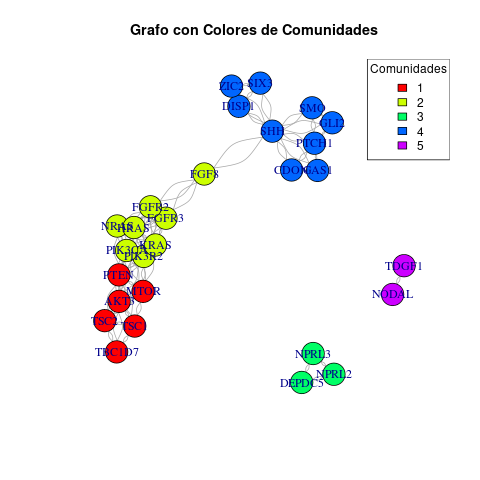
\includegraphics[width=0.8\textwidth]{figures/grafo_colores_comunidades.png}
	\caption{Grafo louvain}
	\label{fig:Grafo_louvain}
\end{figure}

También, se ha obtenido la división por el algoritmo de edge betweenness, que como se ha observado en la Figura \ref{fig:Grafo_between}, son las mismas comunidades pero con una ligera diferencia entre dos comunidades.

\begin{figure}[!]
  \centering
  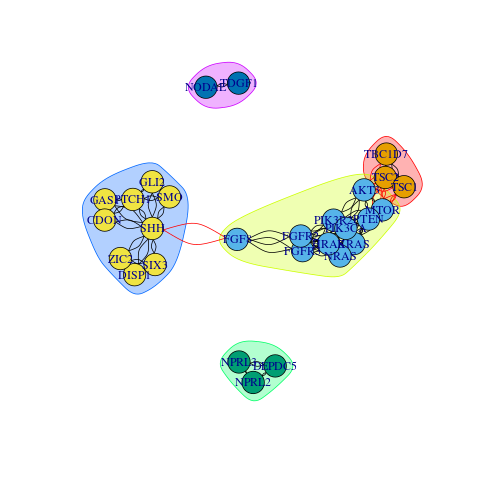
\includegraphics[width=0.8\textwidth]{figures/grafo_alternativo_comunidades.png}
  \caption{Grafo edge betweenness.}
  \label{fig:Grafo_between}
\end{figure}

Para facilitar la comprensión de los diferentes modelos, se muestra en la Tabla \ref{tabla:nodos_enlaces_diferentes} una comparación por nodos. Las filas indican los nodos, la primera columna representa el algoritmo de louvain, y la segunda a la de edge betweenness. Los valores de las celdas indican en que comunidad se encuentra este nodo. Finalmente, en la última columna se muestra si el nodo es asociado a la misma comunidad ("iguales"), o bien si pertenecen a diferentes comunidades ("diferentes").

\newcolumntype{C}{>{\centering\arraybackslash} m{3cm} }
\begin{table}[!]
 	\caption{Descripción de Nodos, Enlaces y Diferentes}
	\centering
	\begin{tabular}{|C|C|C|}
    \toprule
    Nodos & Enlaces & Diferentes \\
    \midrule
     1 & 1 & Iguales \\
     2 & 2 & Iguales \\
     3 & 3 & Iguales \\
    4 & 4 & Iguales \\
     2 & 2 & Iguales \\
     4 & 4 & Iguales \\
    2 & 2 & Iguales \\
     4 & 4 & Iguales \\
     5 & 5 & Iguales \\
     4 & 4 & Iguales \\
     1 & 1 & Iguales \\
     4 & 4 & Iguales \\
     2 & 2 & Iguales \\
     4 & 4 & Iguales \\
     2 & 2 & Iguales \\
     1 & 2 & Diferentes \\
     2 & 2 & Iguales \\
     1 & 2 & Diferentes \\
     2 & 2 & Iguales \\
     1 & 1 & Iguales \\
     3 & 3 & Iguales \\
     1 & 2 & Diferentes \\
     2 & 2 & Iguales \\
     3 & 3 & Iguales \\
    4 & 4 & Iguales \\
     4 & 4 & Iguales \\
     5 & 5 & Iguales \\
     4 & 4 & Iguales \\
 		\bottomrule
   \label{tabla:nodos_enlaces_diferentes}
 	\end{tabular}
\end{table}

Posteriormente, se calculó la modularidad y se representó en la Figura \ref{fig:comparacion_grafos}.

\begin{figure}
  \centering
  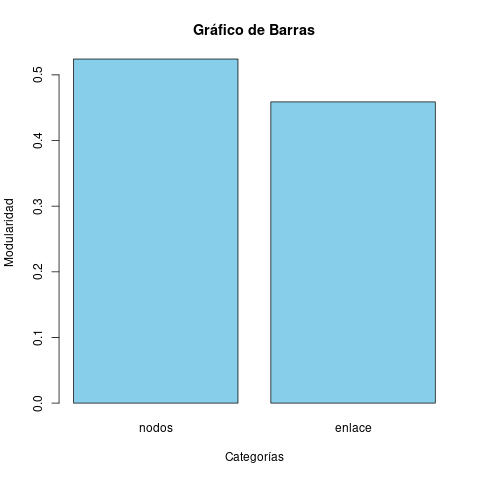
\includegraphics[width=0.8\textwidth]{figures/comparacion_grafos.png}
  \caption{Comparación con modularidad.}
  \label{fig:comparacion_grafos}
\end{figure}

Finalmente, se obtuvo el enriquecimiento funcional del mejor algoritmo basándonos en la modularidad. Para representar las funciones asociadas a cada comunidad, se han creado tantas tablas como comunidades (ver Tablas \ref{tabla:genes_funciones_1}, \ref{tabla:genes_funciones2},  \ref{tabla:genes_funciones3}, \ref{tabla:genes_funciones4} y \ref{tabla:genes_funciones5}), en las que, en la primera columna, se muestra el conjunto de nodos dentro de la comunidad con una función en común, y en la segunda columna, la propia función.

\begin{table}[!]
 	\caption{Descripción de Genes y Funciones de la comunidad 1}
	\centering
	\begin{tabular}{|C|C|}
    \toprule
    \textbf{Genes} & \textbf{Funciones} \\
    \midrule
    TSC2, TSC1, MTOR, PTEN, TBC1D7, AKT3 & negative regulation of intracellular signal transduction (GO:1902532) \\
    \bottomrule
    \label{tabla:genes_funciones_1}
 	\end{tabular}
\end{table}

\begin{table}[!]
 	\caption{Descripción de Genes y Funciones de la comunidad 2}
	\centering
	\begin{tabular}{|C|C|}
    \toprule
    \textbf{Genes} & \textbf{Funciones} \\
    \midrule
    PIK3R2, KRAS, PIK3CA, FGF8, FGFR3, NRAS, HRAS, FGFR2 & MAPK cascade (GO:0000165) \\
    PIK3R2, KRAS, PIK3CA, FGF8, FGFR3, NRAS, HRAS, FGFR2 & Transmembrane receptor protein tyrosine kinase signaling pathway (GO:0007169) \\
    PIK3R2, KRAS, PIK3CA, FGF8, FGFR3, NRAS, HRAS, FGFR2 & Positive regulation of intracellular signal transduction (GO:1902533) \\
    \bottomrule
    \label{tabla:genes_funciones2}
 	\end{tabular}
\end{table}



\begin{table}[!]
 	\caption{Descripción de Genes y Funciones de la comunidad 3}
	\centering
	\begin{tabular}{|C|C|}
    \toprule
    \textbf{Genes} & \textbf{Funciones} \\
    \midrule
    NPRL2, NPRL3, DEPDC5 & Cellular response to amino acid starvation (GO:0034198) \\
    NPRL2, NPRL3, DEPDC5 & Negative regulation of TOR signaling (GO:0032007) \\
    NPRL2, NPRL3, DEPDC5 & Regulation of TOR signaling (GO:0032006) \\
    NPRL2, NPRL3, DEPDC5 & Cellular response to starvation (GO:0009267) \\
    NPRL2, NPRL3, DEPDC5 & Negative regulation of intracellular signal transduction (GO:1902532) \\
    \bottomrule
    \label{tabla:genes_funciones3}
 	\end{tabular}
\end{table}

\begin{table}[!]
 	\caption{Descripción de Genes y Funciones de la comunidad 4}
	\centering
	\begin{tabular}{|C|C|}
    \toprule
    \textbf{Genes} & \textbf{Funciones} \\
    \midrule
    SMO, SIX3, DISP1, SHH, GAS1, PTCH1, GLI2, ZIC2, CDON & Smoothened signaling pathway (GO:0007224) \\
    SMO, SIX3, DISP1, SHH, GAS1, PTCH1, GLI2, ZIC2, CDON & Negative regulation of transcription, DNA-templated (GO:0045892) \\
    \bottomrule
    \label{tabla:genes_funciones4}
 	\end{tabular}
\end{table}



\begin{table}[!]
 	\caption{Descripción de Genes y Funciones de la comunidad 5}
	\centering
	\begin{tabular}{|C|C|}
    \toprule
    \textbf{Genes} & \textbf{Funciones} \\
    \midrule
    NODAL, TDGF1 & BMP signaling pathway (GO:0030509) \\
    NODAL, TDGF1 & Cellular response to BMP stimulus (GO:0071773) \\
    NODAL, TDGF1 & Transmembrane receptor protein serine/threonine kinase signaling pathway (GO:0007178) \\
    NODAL, TDGF1 & Positive regulation of protein phosphorylation (GO:0001934) \\
    NODAL, TDGF1 & Positive regulation of cell proliferation (GO:0008284) \\
    NODAL, TDGF1 & Regulation of apoptotic process (GO:0042981) \\
    NODAL, TDGF1 & Regulation of transcription from RNA polymerase II promoter (GO:0006357) \\
    \bottomrule
    \label{tabla:genes_funciones5}
 	\end{tabular}
\end{table}





	\section{Discusión}

\subsection{Limitaciones}
Una limitación significativa de este proyecto reside en la falta de sujetos humanos reales para estudiar la megalencefalia. Dada la naturaleza de nuestro enfoque, nos basamos en datos y simulaciones, sin contar con la participación directa de individuos afectados. Aunque se ha empleado un enfoque riguroso utilizando modelos y datos disponibles, la ausencia de casos clínicos reales podría afectar la generalización de los resultados a situaciones específicas de pacientes con megalencefalia. Se recomienda cautela al extrapolar los hallazgos a poblaciones humanas y se sugiere la validación adicional mediante estudios clínicos con participantes reales en futuras investigaciones. 

	\section{Conclusiones}

Este estudio sobre la megalencefalia se ha desarrollado una metodología gracias a la cual se han detectado nuevos genes que ha permitido identificar y comprender mejor las limitaciones y desafíos en el enfoque de estudio acerca de la enfermedad cerebral. Los resultados obtenidos a través del enriquecimiento funcional y análisis de redes, como se ha sospechado por los nuevos avances sobre los fundamentos moleculares de este trastorno, han permitido descubrir nuevas conexiones y patrones entre la enfermedad y sus síntomas, lo que puede ser de gran ayuda para los médicos en el diagnóstico y tratamiento de la megalencefalia. Además, el uso de herramientas avanzadas de análisis de redes puede ser aplicado en otros ámbitos de la medicina, lo que puede conducir a avances importantes en el cuidado y tratamiento de diversas enfermedades. Así, este estudio representa un importante avance en la comprensión de la megalencefalia y sus implicaciones clínicas, ya que se ha descubierto que parte de los genes propuestos en la red son genes ya conocidos y relacionados con la enfermedad de manera experimental. 
	
	
	%%%%%%%%%%%%%%%%%%%%%%%%%%%%%%%%%%%%%%%%%%%%%%
	%% OTRA INFORMACIÓN                         %%
	%%%%%%%%%%%%%%%%%%%%%%%%%%%%%%%%%%%%%%%%%%%%%%
	
	\begin{backmatter}
	
		% \section*{Abreviaciones}%% No hay ninguna, creo
		
		\section*{Disponibilidad de datos y materiales}%% if any
			GitHub: \url{https://github.com/FlorinUMA/biologia_sistemas}
		
		\section*{Contribución de los autores}
			C.V.R: Responsable parcial de la creación del código de R, redactora de la metodología y parte de la discusión.\\
			F.B.V: Responsable de la creación del código de Python, gestión de bibliografías, pruebas y supervisión de la automatización, redacción del abstract, conclusión y revisor general del documento.\\
			M.A.R.V: Responsable de generar todo el flujo de trabajo en el script de bash y moldear los archivos de código al mismo. Además de la contribución en diversas partes del proyecto como introducción o discusión.\\
			R.O.B: Encargado de creación de código de Python y R, resultados y aportaciones en discusión e introducción.
			
		
		
		%%%%%%%%%%%%%%%%%%%%%%%%%%%%%%%%%%%%%%%%%%%%%%%%%%%%%%%%%%%%%%%%%%%%%%%%%%%%%%%%%%%%%%%%
		%% BIBLIOGRAFIA: no teneis que tocar nada, solo sustituir el archivo bibliography.bib %%
		%% por el que hayais generado vosotros                                                %%
		%%%%%%%%%%%%%%%%%%%%%%%%%%%%%%%%%%%%%%%%%%%%%%%%%%%%%%%%%%%%%%%%%%%%%%%%%%%%%%%%%%%%%%%%
		
		\bibliographystyle{bmc-mathphys} % Style BST file (bmc-mathphys, vancouver, spbasic).
		\bibliography{bibliography/references}      % Bibliography file (usually '*.bib' )
	
	\end{backmatter}
\end{document}
